\documentclass[a4paper, 12pt]{article}

%\usepackage{savetrees}
\usepackage{graphicx}
\graphicspath{{./images/}}
\title {Student Robotics 2009\\ Slug Documentation}
\date{\today}
\setcounter{tocdepth}{1}


\begin {document}

\maketitle

\noindent This document describes the functions of the Slug

\section{Board Outline}

\begin{figure}[ht]
\begin{center}
\includegraphics[keepaspectratio, width=12cm]{./images/outline.png}
\caption{\label{slug-outline}The board outline of the slug}
\end{center}
\end{figure}

\section{Brief Description}

\clearpage
\newpage

\section {Pin out}

\begin{figure}[ht]
\begin{center}
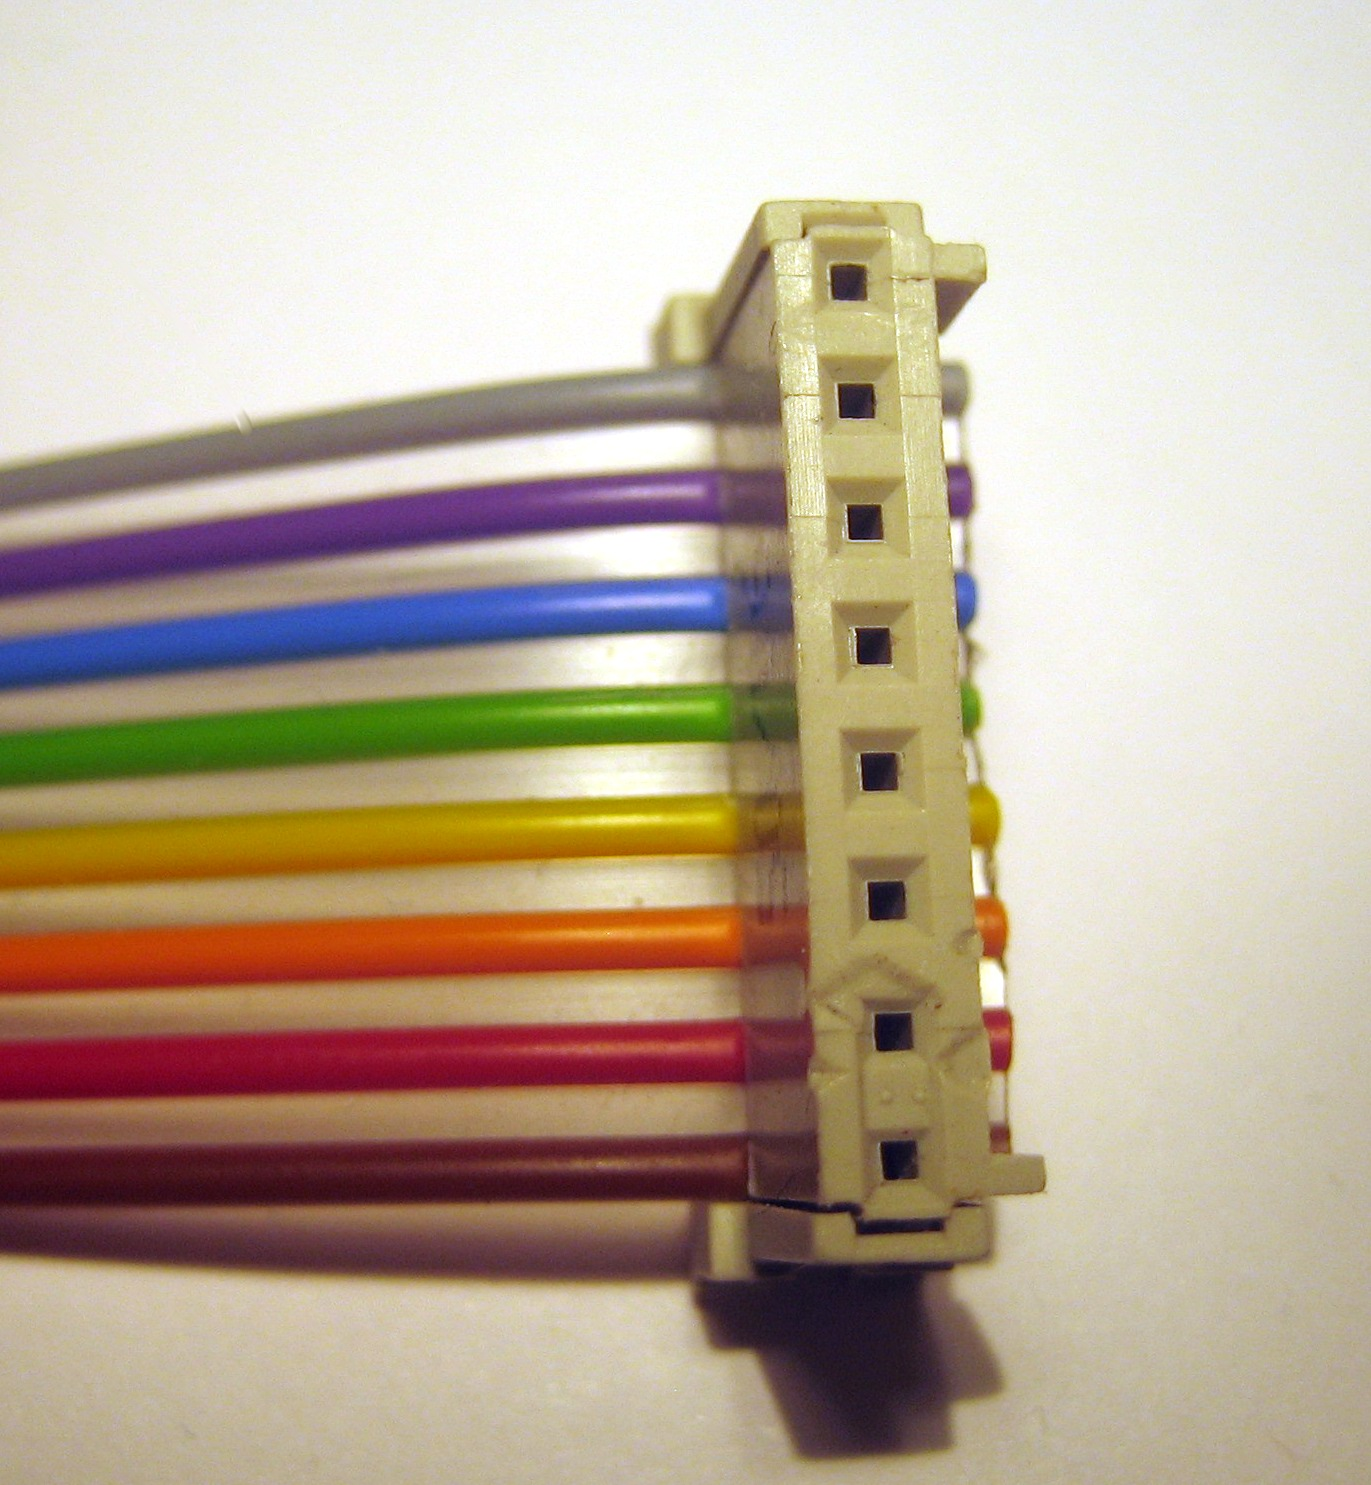
\includegraphics[keepaspectratio, width=7cm]{./images/slugpins.png}
\caption {\label{slug-pinout}Slug pin-out}
\end{center}
\end{figure}

\begin{center}
\begin{tabular}{|c|c|c|}
\hline
\textbf {Pin Number} & \textbf {Wire Colour} & \textbf {Description}\\
\hline
1 & Grey & GND\\
2 & SCL & Violet\\
3 & SDA & Blue\\
4 & Xbee to Slug & Green\\
5 & Slug to Xbee & Yellow\\
6 & Slug Boot Pin & Orange\\
7 & VREGSLUG2 & Red\\
Not Connected & Not used & Brown\\
\hline
\end{tabular}
\end{center}

\end {document}
